\documentclass{article}
\usepackage[utf8]{inputenc}
\usepackage[a4paper, total={6.5in, 10.5in}]{geometry}
\usepackage{merriweather}
\usepackage[hidelinks]{hyperref}
\usepackage{graphicx}
\usepackage{xcolor}
\renewcommand{\baselinestretch}{1.22} 

% for markdown inline code effect
\definecolor{bgcolor}{HTML}{E0E0E0}
\let\oldtexttt\texttt
\renewcommand{\texttt}[1]{
  \colorbox{bgcolor}{\oldtexttt{#1}}
  }
 
% % removing word break stuff
\tolerance=1
\emergencystretch=\maxdimen
\hyphenpenalty=10000
\hbadness=10000

\title{CS315: Lab Assignment 2}
\author{
  B Siddharth Prabhu\\
  \href{mailto:200010003@iitdh.ac.in}{\texttt{200010003@iitdh.ac.in}}
  }
\date{10 January 2023}

\begin{document}

\maketitle

\section{Answers for Part 1: Wireshark Basics}

\subsection*{(1) If a packet is highlighted by black, what does it mean for the packet?}
By default, black highlighting of packets indicates \underline{TCP packets with problems}. In the below screenshot, we observe that some such problems are `TCP ACKed unseen segment' (This acknowledges data that wasn't captured) and `TCP Previous segment not captured' (This means that Wireshark is seeing an acknowledgment for a packet that it hasn't captured).

\begin{figure}[!hbt]
    \centering
    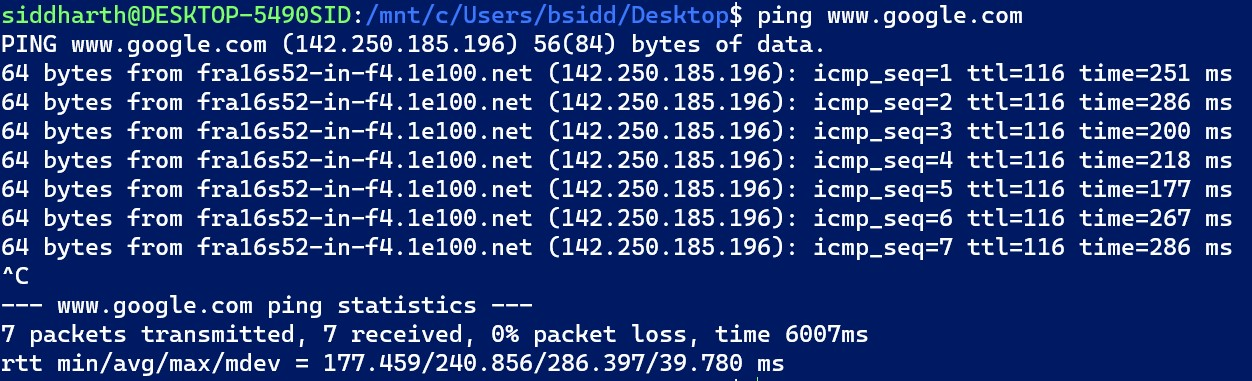
\includegraphics[scale=0.6]{q1a.jpg}
    \caption{Black highlighting}
    \label{fig:my_label1}
\end{figure}

\subsection*{(2) What is the filter command for listing all outgoing HTTP traffic?}
Outgoing HTTP traffic consists of HTTP requests, that may be GET or POST. We would like to view all of them, so the filter command is the following:\\ \vspace{2mm}
\fbox{ \begin{minipage}{45.5em}
http.request
\end{minipage}
}


\subsection*{(3) Why does DNS use Follow UDP Stream while HTTP use Follow TCP Stream?}
UDP (User Datagram Protocol) is a connection-less protocol used to send smaller segments of data on a network, while TCP (Transmission Control Protocol) is a connection-oriented protocol used to send data packets along a network connection.

DNS requests are tiny, and fit in UDP segments easily. Also, we want Domain Name Resolution to occur quickly, so using UDP stream would be a better choice for this purpose. Hence, the main reason for this is \underline{performance}.

HTTP uses the more reliable TCP stream, since the files, images, and other data that we get from the remote host must not be dropped along the way. Although HTTP could technically use UDP, if a UDP packet containing the first part of a web page is lost, then it is not retransmitted. Then, the application layer would have to handle this. To avoid such overhead burdens, it is better to use TCP instead. Hence, the main reason for this is \underline{reliability}.




\section{Answers for Task 2: Wireshark for Packet Capture and Analysis}

\subsection*{(1) List the different protocols that appear in the protocol column in the unfiltered packet-listing window in wireshark GUI?}
\begin{itemize}
    \item TCP : Transmission Control Protocol
    \item HTTP : HyperText Transfer Protocol
    \item ARP : Address Resolution Protocol
    \item QUIC : Quick UDP Internet Connections
    \item TLSv1.2 : Transport Layer Security (Version 1.2)
    \item ICMPv6 : Internet Control Message Protocol for IPv6
    \item NTP : Network Time Protocol
    \item DNS : Domain Network System (a.k.a. Domain Name System)
    \item SSDP : Simple Service Discovery Protocol
\end{itemize}

\subsection*{(2) How long did it take from when the HTTP GET message was sent until the HTTP OK reply was received for the web page you visited in your web browser? 
% (By default, the value of the Time column in the packet-listing window is the amount of time, in seconds, since Wireshark tracing began. To display the Time field in time-of-day format, select the Wireshark View pull down menu, then select Time Display Format, then select Time-of-day.)
}
This can be easily obtained by clicking on the HTTP GET record and setting time reference, or by manually subtracting time values. The obtained time difference in this case is \underline{0.197771514 seconds}.

\begin{figure}[!hbt]
    \centering
    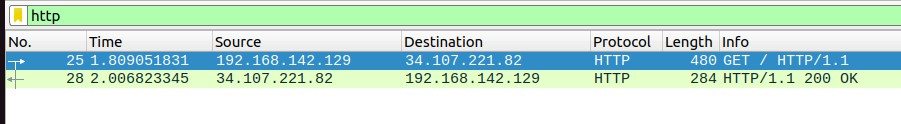
\includegraphics[scale=0.95]{http-ok.jpg}
    \caption{Without Setting Time Reference}
    \label{fig:my_labe223l}
\end{figure}
\begin{figure}[!hbt]
    \centering
    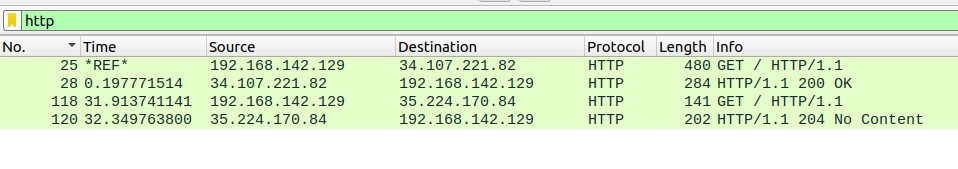
\includegraphics[scale=0.9]{http-ok-ref.jpg}
    \caption{With Setting Time Reference}
    \label{fig:my_labe22dd3l}
\end{figure}

\subsection*{(3) What is the Internet (IP) address of the URL you visited and what is the Internet address of your computer?}

\fbox{ \begin{minipage}{45.5em}
IP address of URL visited: 34.107.221.82 \\
IP address of my computer: 192.168.142.129 \\
Note that this is being run on an Ubuntu Virtual Machine.
\end{minipage}
}


\subsection*{(4) Print the two HTTP messages displayed in wireshark GUI after you had visited the above URL through your web browser. To do so, select Print from the Wireshark File command menu, and select “Selected Packet Only” and then click Print.}
\begin{figure}[!hbt]
    \centering
    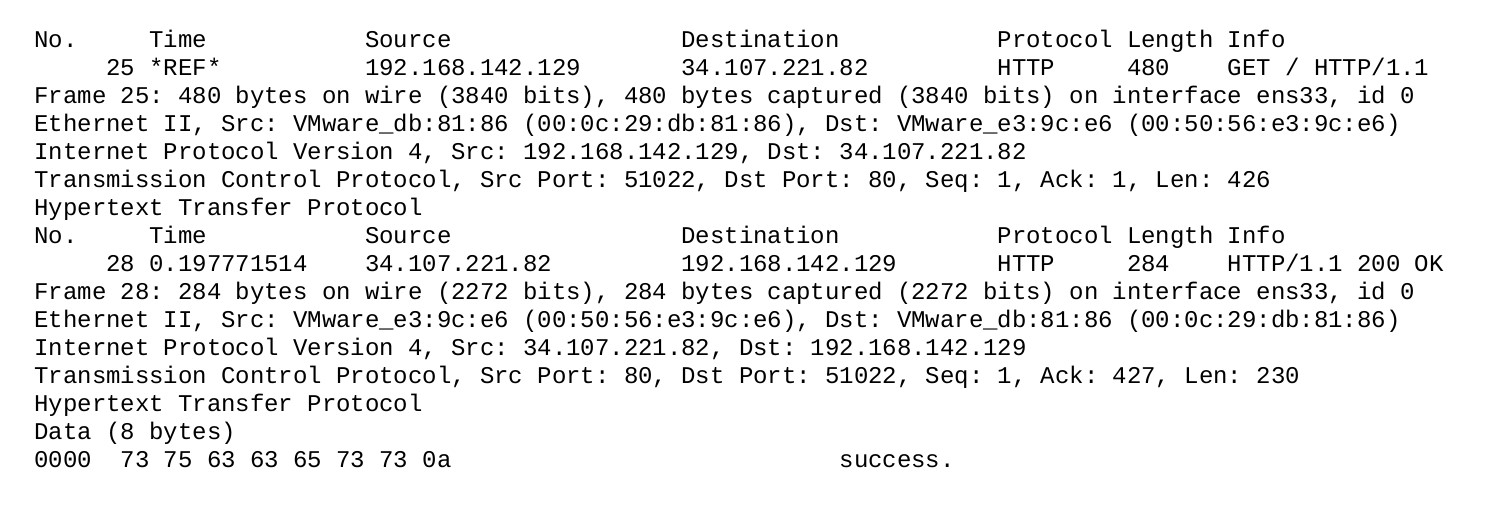
\includegraphics[scale=0.6]{printed.jpg}
    \caption{HTTP messages}
    \label{fig:my_labe22jdd3l}
\end{figure}

\subsection*{(5) Execute the above steps on Google Chrome, Safari or any other browsers also, check whether you will be able to see http protocol. Write down your analysis with screenshots.}
So far, Google Chrome was used. With Mozilla Firefox, the following is obtained:

\begin{figure}[!hbt]
    \centering
    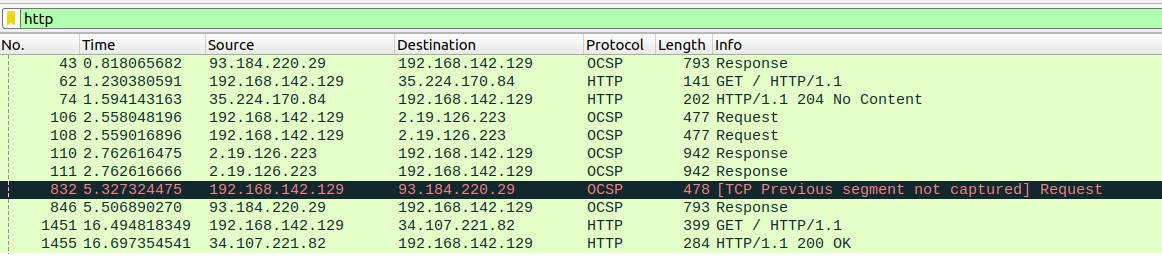
\includegraphics[scale=0.8]{firefox.jpg}
    \caption{HTTP protocol with Firefox}
    \label{fig:my_labe22jdd3l}
\end{figure}

Hence, Mozilla Firefox also uses HTTP Protocol, and the same can be viewed in Wireshark. 

Also, I have tried the same on Windows, with Chrome as browser. The obtained records are as follows
\begin{figure}[!hbt]
    \centering
    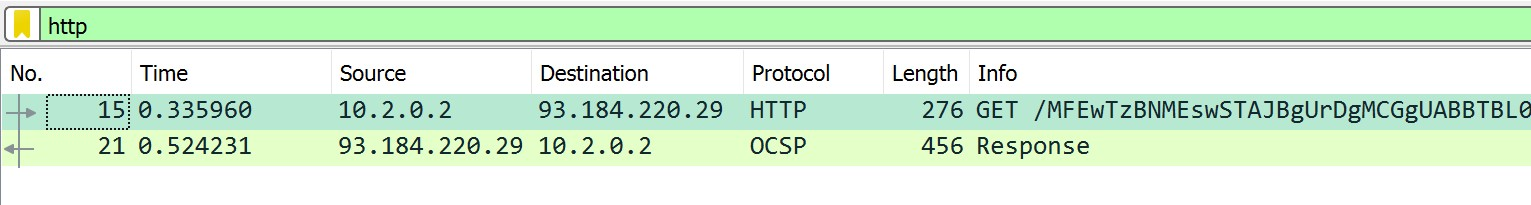
\includegraphics[scale=0.6]{wind.jpg}
    \caption{Using Windows}
    \label{fig:my_labe2jj2jdd3l}
\end{figure}

\end{document}
